\documentclass[../../cjSOE.tex]{subfiles}
% \usepackage{url}
% \usepackage{natbib}
% \usepackage{csvsimple}
% \usepackage{graphicx}
% \usepackage[flushleft]{threeparttable}
% \usepackage{color}
% \usepackage{amsmath,amssymb}
% \usepackage{moreverb}
% \usepackage{caption}
% \usepackage{multirow}

\begin{document}
\begin{verbatimwrite}{../../insert_saving-and-uncert}
\subsection{Robustness Check}

In this section, we show that the positive relationship between income uncertainty and the aggregate saving rate holds in a model with more realistic settings than the basic tractable model. Specifically, we use the model in \cite{cstwMPC} (henceforth 'CSTW'), which incorporates transitory and permanent shocks {\it a la} \cite{friedmanATheory} calibrated to match empirical estimates of such shocks in U.S.\ data.  We use this model to calculate a quantitative relationship between uncertainty and precautionary saving.  

In the basic model, the only uncertainty comes from the shock of becoming unemployed. Here household income $y_{t}$ is determined by the aggregate wage rate $W_{t}$ and two idiosyncratic components, the permanent component $p_{t}$ and the transitory shock $\tshk_{t}$:
\begin{align}
y_{t}=p_{t}\tshk_{t}{W}_{t}
\end{align}
The permanent component follows:
\begin{align}
p_{t}=p_{t-1}\permShk_{t}
\end{align}
The transitory component is:
\begin{eqnarray}
  \xi_{t} & = & \mu \textrm{ with probability }\ \urate_{t}, \label{eq:tran}
\\ & = & (1-\tau_{t})\ell\theta_{t} \textrm{ with probability }\ 1-\urate_{t}, \nonumber
\end{eqnarray}
Here $\mu$ is the unemployment insurance payment when unemployed. $\tau_{t}$ is the rate of tax collected to pay unemployment benefits, $\ell$ is time worked per employee. $\permShk$ and $\theta$ are white noise drawn from log normal distribution and $\mathbb{E}_{t}\permShk_{t+n}=\mathbb{E}_{t}\theta_{t+n}=1\forall n>0$. By changing the value of $\sigma_{\permShk}$ and $\sigma_{\theta}$. we change the degree of uncertainty faced by households.The details of the model are described in appendix A.7

%In this model, the economy consists of a continuum of households of mass one distributed on the unit interval. Households die with a constant probability $D=1-\PLives$ between periods. This is different from the baseline model in which households only face probability of dying after they become unemployed. Each household maximize expected discount utility from consumption:
%\begin{eqnarray}
%\max\mathbb{E}_{t}\sum_{n=0}^{\infty}(\PLives\beta)^{n}\util(\cFunc_{t+n})
%\end{eqnarray}
%The household consumption functions satisfies:
%\begin{eqnarray}
%v(m_{t}) & = & \max_{c_{t}} \mathbb{E}_{t}\sum_{n=0}^{\infty}(\PLives\beta)^{n}\util(\cFunc_{t+n}), \label{eq:tran}
%\\ \text{s.t.}, \nonumber
%\\a_{t} & = & m_{t}-\c(m_{t})
%\\k_{t+1} & = & \frac{a_{t}}{\PLives \permShk_{t+1}}
%\\m_{t+1} & = & (\DeprFac+r_{t})k_{t+1}+\tshk_{t+1}
%\\a_{t} & \geq & 0
%\end{eqnarray}
%The production function is Cobb-Douglass:
%\begin{align}
%\end{align}
%The aggregate wage rate $W_{t}$ is determined by the aggregate productivity $Z_{t}$, capital stock $K_{t}$, and the aggregate supply of labor $L_{t}$:
%\begin{align}
%\end{align}
%$L_{t}$ is driven by two aggregate shocks:
%\begin{align}
%\\P_{t}=P_{t-1}\Psi_{t}
%\end{align}
%where $P_{t}$ is aggregate permanent productivity, 	$\Psi_{t}$ is the aggregate permanent shock
%and $\Theta_{t}$ is the aggregate transitory shock.\footnote{Note that $\Psi$ is the capitalized version of the Greek letter $\psi$ used for the idiosyncratic permanent shock; similarly $\Theta$ is the capitalized $\theta$}

The parameters are calibrated as in CSTW except for aggregate productivity growth rate and individual productivity growth rate. In CSTW, there is no aggregate and individual productivity growth; here we allow aggregate productivity growth $G=1.015$, and individual productivity growth $X=1.01$.

CSTW find that in order for the model to generate a plausible distribution of wealth it is necessary to build in some form of \textit{ex ante} hetergogeneity; we follow them in assuming that the time preference rate is the locus of heterogeneity. We calibrate the mean of the time discount factor to match the U.S.\ aggregate wealth to income ratio and the distribution of the time discount factor to match the wealth distribution among households in U.S.\ data.\footnote{The wealth to income ratio and wealth distribution data are obtained from the Survey of Consumer Finances.}

%\begin{eqnarray}
%a_{t} & = & m_{t}-\c(m_{t}), \label{eq:cons1}
%\\ k_{t+1}& = & \frac{a_{t}}{\pLive \permShk_{t+1}}, \label{eq:cons2}
%\end{eqnarray}

Following CSTW, we set the benchmark value of $\sigma_{\psi}^{2}$ and $\sigma_{\theta}^{2}$ to be $0.010\times4/11$ and $0.010\times4$. Under these new model settings, the growth impatience condition needs to be modified to be:

\begin{align}
	\PatPGroAdj = \frac{(\Discount \Rfree)^{1/\CRRA}\PLives}{\PGroAdj}
\end{align}
Where $\PGroAdj=\PGro \acute{\psi}$ and $\acute{\psi}\equiv (\mathbb{E}[\psi^{-1}])^{-1}$. By computing aggregate saving rate while increasing $\sigma_{\psi}^{2}$ and $\sigma_{\theta}^{2}$,  we derive the relationship between aggregate saving rate and the degree of uncertainty. Increasing $\sigma_{\psi}^{2}$ will also cause $\PGroAdj$ to increase. Agents with different $\beta$ have different $\PGroAdj$. The growth impatience condition $\PGroAdj<1$ of the most patient agent restricts the maximum value of $\sigma_{\psi}^{2}$ we can choose. Here we allow $\sigma_{\psi}^{2}$ and $\sigma_{\theta}^{2}$ to move from half of their benchmark values to twice the benchmark value.  Figure \ref{figure:savings} shows how the aggregate saving rate changes with $\sigma_{\psi}$. The first row in Table 2 reports the slope and $R^2$ calculated from OLS regression between the aggregate saving rate and the standard deviation of the permanent income shock. Under the model calibration, aggregate saving rate is almost perfectly correlated with the standard deviation of $\sigma_{\psi}$: adding 0.01 to $\sigma_{\psi}$ will cause the aggregate savings rate to rise about 0.83 percent. Figure \ref{figure:savingsTran} shows how the aggregate saving rate varies with the standard deviation of the transitory income shock. The regression result is reported in the second row of Table 2. The impact of transitory uncertainty is much smaller than the impact of permanent uncertainty. Increasing  $\sigma_{\theta}$ by 0.01 will cause the aggregate saving rate to increase by 0.011 percent. The last column reports the growth impatience factor of the most patient agent when $\sigma_{\psi}^{2}$ reaches its upper limit in each of the two exercises. We can see that the growth impatience condition is well satisfied in both exercises.
%\PatPGro
\begin{table}
	\centerline{\bf Table 2}
	\label{tab:Uncert}
	\begin{center}
		\begin{tabular}{ c c c c }
			\hline
			~ & Slope & $R^2$ & max $\PatPGro$\\
			\hline 
			\multirow{2}{4em}{$\sigma_{\Psi}$} & 0.826 & \multirow{2}{*}{0.998} & \multirow{2}{4em}{0.998}\\
			& ($9.1\times10^{-3}$)***\\
			\multirow{2}{4em}{$\sigma_{\theta}$} & 0.0111 & \multirow{2}{*}{0.989} & \multirow{2}{4em}{0.996}\\
			& ($3.1\times10^{-4}$)***\\
			\hline
		\end{tabular}
		\\
	\end{center}
	\begin{tablenotes}
		\small
		\item Table 2 presents the correlation between the aggregate saving rate and the degree of income uncertainty. The first two columns show the slope and $R^2$ result from OLS regression. The third column show the growth impatience factor of the most patient agent in the economy. The first row shows the result of OLS regression between the aggregate saving rate and the standard deviation of permanent income shocks $\sigma_{\psi}$. The second row shows the result of OLS regression between the aggregate saving rate and the standard deviation of transitory income shocks $\sigma_{\theta}$. Standard errors are reported in parenthesis. ***represents significance level of 0.01. 
	\end{tablenotes}
\end{table}

\begin{figure}[h]
	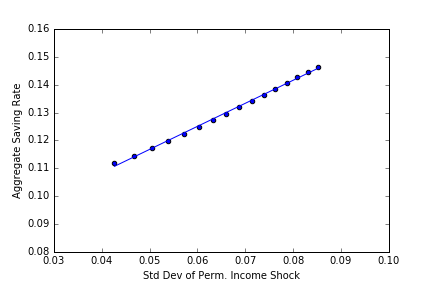
\includegraphics[scale=0.8]{\econtexRoot/LaTeX/Insertions/SavingVSPermShr_Youth_MPC_15.png}
	\centering
	\caption{Change in Savings Following increasing in Permanent Income Uncertainty}
	\label{figure:savings}
	
	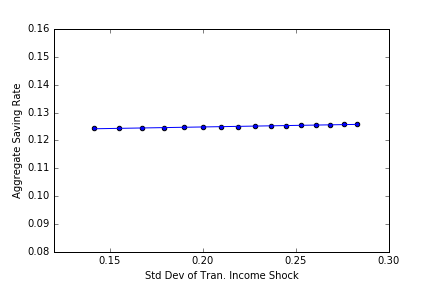
\includegraphics[scale=0.8]{\econtexRoot/LaTeX/Insertions/SavingVSTranShr_Youth_MPC_15.png}
	\centering
	\caption{Change in Savings Following increasing in Transitory Income Uncertainty}
	\label{figure:savingsTran}
\end{figure}

\end{verbatimwrite}
\subsection{Robustness Check}

In this section, we show that the positive relationship between income uncertainty and the aggregate saving rate holds in a model with more realistic settings than the basic tractable model. Specifically, we use the model in \cite{cstwMPC} (henceforth 'CSTW'), which incorporates transitory and permanent shocks {\it a la} \cite{friedmanATheory} calibrated to match empirical estimates of such shocks in U.S.\ data.  We use this model to calculate a quantitative relationship between uncertainty and precautionary saving.

In the basic model, the only uncertainty comes from the shock of becoming unemployed. Here household income $y_{t}$ is determined by the aggregate wage rate $W_{t}$ and two idiosyncratic components, the permanent component $p_{t}$ and the transitory shock $\tshk_{t}$:
\begin{align}
y_{t}=p_{t}\tshk_{t}{W}_{t}
\end{align}
The permanent component follows:
\begin{align}
p_{t}=p_{t-1}\permShk_{t}
\end{align}
The transitory component is:
\begin{eqnarray}
  \xi_{t} & = & \mu \textrm{ with probability }\ \urate_{t}, \label{eq:tran}
\\ & = & (1-\tau_{t})\ell\theta_{t} \textrm{ with probability }\ 1-\urate_{t}, \nonumber
\end{eqnarray}
Here $\mu$ is the unemployment insurance payment when unemployed. $\tau_{t}$ is the rate of tax collected to pay unemployment benefits, $\ell$ is time worked per employee. $\permShk$ and $\theta$ are white noise drawn from log normal distribution and $\mathbb{E}_{t}\permShk_{t+n}=\mathbb{E}_{t}\theta_{t+n}=1\forall n>0$. By changing the value of $\sigma_{\permShk}$ and $\sigma_{\theta}$. we change the degree of uncertainty faced by households.The details of the model are described in appendix A.7

%In this model, the economy consists of a continuum of households of mass one distributed on the unit interval. Households die with a constant probability $D=1-\PLives$ between periods. This is different from the baseline model in which households only face probability of dying after they become unemployed. Each household maximize expected discount utility from consumption:
%\begin{eqnarray}
%\max\mathbb{E}_{t}\sum_{n=0}^{\infty}(\PLives\beta)^{n}\util(\cFunc_{t+n})
%\end{eqnarray}
%The household consumption functions satisfies:
%\begin{eqnarray}
%v(m_{t}) & = & \max_{c_{t}} \mathbb{E}_{t}\sum_{n=0}^{\infty}(\PLives\beta)^{n}\util(\cFunc_{t+n}), \label{eq:tran}
%\\ \text{s.t.}, \nonumber
%\\a_{t} & = & m_{t}-\c(m_{t})
%\\k_{t+1} & = & \frac{a_{t}}{\PLives \permShk_{t+1}}
%\\m_{t+1} & = & (\DeprFac+r_{t})k_{t+1}+\tshk_{t+1}
%\\a_{t} & \geq & 0
%\end{eqnarray}
%The production function is Cobb-Douglass:
%\begin{align}
%\end{align}
%The aggregate wage rate $W_{t}$ is determined by the aggregate productivity $Z_{t}$, capital stock $K_{t}$, and the aggregate supply of labor $L_{t}$:
%\begin{align}
%\end{align}
%$L_{t}$ is driven by two aggregate shocks:
%\begin{align}
%\\P_{t}=P_{t-1}\Psi_{t}
%\end{align}
%where $P_{t}$ is aggregate permanent productivity, 	$\Psi_{t}$ is the aggregate permanent shock
%and $\Theta_{t}$ is the aggregate transitory shock.\footnote{Note that $\Psi$ is the capitalized version of the Greek letter $\psi$ used for the idiosyncratic permanent shock; similarly $\Theta$ is the capitalized $\theta$}

The parameters are calibrated at the same level as they are in CSTW except for aggregate productivity growth rate and individual productivity growth rate. In CSTW, there is no aggregate and individual productivity growth; here we allow aggregate productivity growth $G=1.015$, and individual productivity growth $X=1.01$.

CSTW find that in order for the model to generate a plausible distribution of wealth it is necessary to build in some form of \textit{ex ante} hetergogeneity; we follow them in assuming that the time preference rate is the locus of heterogeneity. We calibrate the mean of the time discount factor to match the U.S.\ aggregate wealth to income ratio and the distribution of the time discount factor to match the wealth distribution among households in U.S.\ data.\footnote{The wealth to income ratio and wealth distribution data are obtained from the Survey of Consumer Finances.}

%\begin{eqnarray}
%a_{t} & = & m_{t}-\c(m_{t}), \label{eq:cons1}
%\\ k_{t+1}& = & \frac{a_{t}}{\pLive \permShk_{t+1}}, \label{eq:cons2}
%\end{eqnarray}

Following CSTW, we set the benchmark value of $\sigma_{\psi}^{2}$ and $\sigma_{\theta}^{2}$ to be $0.010\times4/11$ and $0.010\times4$. Under these new model settings, the growth impatience condition needs to be modified to be:

\begin{align}
	\PatPGroAdj = \frac{(\Discount \Rfree)^{1/\CRRA}\PLives}{\PGroAdj}
\end{align}
Where $\PGroAdj=\PGro \acute{\psi}$ and $\acute{\psi}\equiv (\mathbb{E}[\psi^{-1}])^{-1}$. By computing aggregate saving rate while increasing $\sigma_{\psi}^{2}$ and $\sigma_{\theta}^{2}$,  we derive the relationship between aggregate saving rate and the degree of uncertainty. Increasing $\sigma_{\psi}^{2}$ will also cause $\PGroAdj$ to increase. Agents with different $\beta$ have different $\PGroAdj$. The growth impatience condition $\PGroAdj<1$ of the most patient agent restricts the maximum value of $\sigma_{\psi}^{2}$ we can choose. Here we allow $\sigma_{\psi}^{2}$ and $\sigma_{\theta}^{2}$ to move from half of their benchmark values to twice the benchmark value.  Figure \ref{figure:savings} shows how the aggregate saving rate changes with $\sigma_{\psi}$. The first row in Table 2 reports the slope and $R^2$ calculated from OLS regression between the aggregate saving rate and the standard deviation of the permanent income shock. Under the model calibration, aggregate saving rate is almost perfectly correlated with the standard deviation of $\sigma_{\psi}$: adding 0.01 to $\sigma_{\psi}$ will cause the aggregate savings rate to rise about 0.83 percent. Figure \ref{figure:savingsTran} shows how the aggregate saving rate varies with the standard deviation of the transitory income shock. The regression result is reported in the second row of Table 2. The impact of transitory uncertainty is much smaller than the impact of permanent uncertainty. Increasing  $\sigma_{\theta}$ by 0.01 will cause the aggregate saving rate to increase by 0.011 percent. The last column reports the growth impatience factor of the most patient agent when $\sigma_{\psi}^{2}$ reaches its upper limit in each of the two exercises. We can see that the growth impatience condition is well satisfied in both exercises.
%\PatPGro
\begin{table}
	\centerline{\bf Table 2}
	\label{tab:Uncert}
	\begin{center}
		\begin{tabular}{ c c c c }
			\hline
			~ & Slope & $R^2$ & max $\PatPGro$\\
			\hline
			\multirow{2}{4em}{$\sigma_{\Psi}$} & 0.826 & \multirow{2}{*}{0.998} & \multirow{2}{4em}{0.998}\\
			& ($9.1\times10^{-3}$)***\\
			\multirow{2}{4em}{$\sigma_{\theta}$} & 0.0111 & \multirow{2}{*}{0.989} & \multirow{2}{4em}{0.996}\\
			& ($3.1\times10^{-4}$)***\\
			\hline
		\end{tabular}
		\\
	\end{center}
	\begin{tablenotes}
		\small
		\item Table 2 presents the correlation between the aggregate saving rate and the degree of income uncertainty. The first two columns show the slope and $R^2$ result from OLS regression. The third column show the growth impatience factor of the most patient agent in the economy. The first row shows the result of OLS regression between the aggregate saving rate and the standard deviation of permanent income shocks $\sigma_{\psi}$. The second row shows the result of OLS regression between the aggregate saving rate and the standard deviation of transitory income shocks $\sigma_{\theta}$. Standard errors are reported in parenthesis. ***represents significance level of 0.01.
	\end{tablenotes}
\end{table}

\begin{figure}[h]
	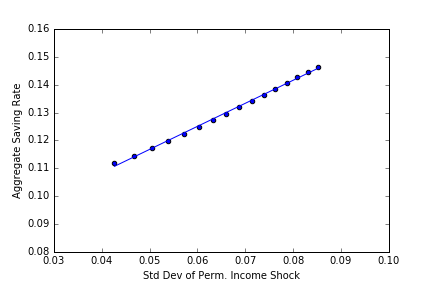
\includegraphics[scale=0.8]{\econtexRoot/LaTeX/Insertions/SavingVSPermShr_Youth_MPC_15.png}
	\centering
	\caption{Change in Savings Following increasing in Permanent Income Uncertainty}
	\label{figure:savings}

	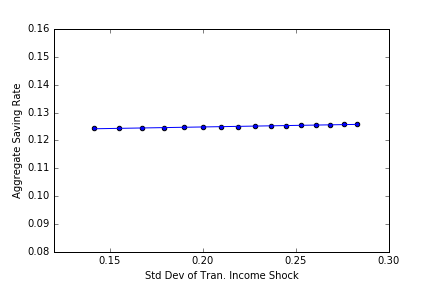
\includegraphics[scale=0.8]{\econtexRoot/LaTeX/Insertions/SavingVSTranShr_Youth_MPC_15.png}
	\centering
	\caption{Change in Savings Following increasing in Transitory Income Uncertainty}
	\label{figure:savingsTran}
\end{figure}



\bibliographystyle{ier}
\bibliography{economics,Reference}
\end{document}
